\documentclass{standalone}
\usepackage{graphicx}	
\usepackage{amssymb, amsmath}
\usepackage{color}

\usepackage{tikz}
\usetikzlibrary{intersections, backgrounds}

\definecolor{light}{RGB}{220, 188, 188}
\definecolor{mid}{RGB}{185, 124, 124}
\definecolor{dark}{RGB}{143, 39, 39}
\definecolor{highlight}{RGB}{180, 31, 180}
\definecolor{gray10}{gray}{0.1}
\definecolor{gray20}{gray}{0.2}
\definecolor{gray30}{gray}{0.3}
\definecolor{gray40}{gray}{0.4}
\definecolor{gray60}{gray}{0.6}
\definecolor{gray70}{gray}{0.7}
\definecolor{gray80}{gray}{0.8}
\definecolor{gray90}{gray}{0.9}
\definecolor{gray95}{gray}{0.95}

\newcommand*{\offset}{0.025}

\begin{document}

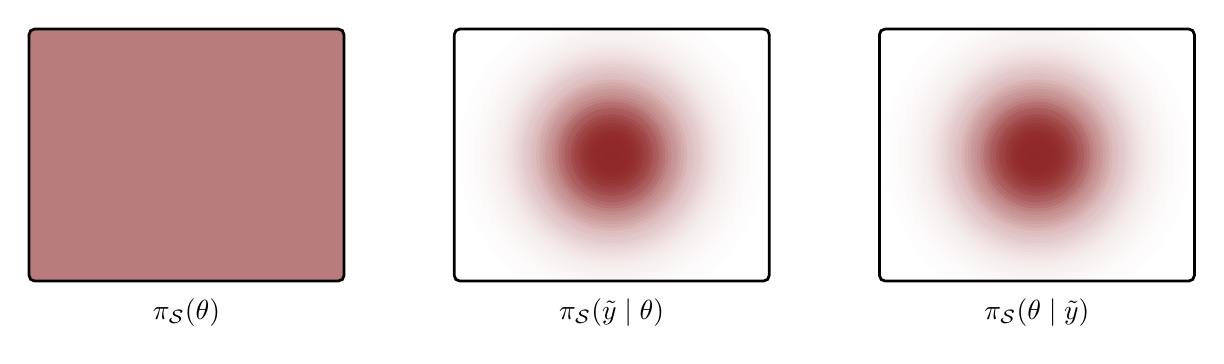
\begin{tikzpicture}[scale=0.2, thick] 
  % Prior
  \pgfmathsetmacro{\dx}{-27}
  \fill [rounded corners=2pt, color=mid] (-10 + \dx, -6) rectangle (10 + \dx, 10);
  \draw [rounded corners=2pt, color=black, line width=1] (-10 + \dx, -6) rectangle (10 + \dx, 10);
  \node [] at (0 + \dx, -8) { $\pi_{\mathcal{S}}(\theta)$ };
      
  % Likelihood               
  \pgfmathsetmacro{\dx}{0}
  
  \begin{scope}
    \clip (-10 + \dx, -6) rectangle (10 + \dx, 10); 
    \foreach \i in {0.1, 0.2, ..., 5} {
      \fill[opacity={exp(-1.25 * \i)}, dark] (0 + \dx, 2) circle ({2 * \i});      
    }
  \end{scope}
  
  \draw [rounded corners=2pt, color=black, line width=1] (-10 + \dx, -6) rectangle (10 + \dx, 10);
  \node [] at (0 + \dx, -8) { $\pi_{\mathcal{S}}(\tilde{y} \mid \theta)$ };
          
  % Posterior           
  \pgfmathsetmacro{\dx}{+27}
  
    \begin{scope}
    \clip (-10 + \dx, -6) rectangle (10 + \dx, 10); 
    \foreach \i in {0.1, 0.2, ..., 10} {
      \fill[opacity={exp(-1.25 * \i)}, dark] (0 + \dx, 2) circle ({2 * \i});       
    }
  \end{scope}
  
  \draw [rounded corners=2pt, color=black, line width=1] (-10 + \dx, -6) rectangle (10 + \dx, 10);
  \node [] at (0 + \dx, -8) { $\pi_{\mathcal{S}}(\theta \mid \tilde{y})$ };
\end{tikzpicture}

\end{document}   